\documentclass[a4paper]{iacas}

\usepackage{cite}
\usepackage{hyperref}% embedding hyperlinks [must be loaded after dropping]
\usepackage{amsmath,amsthm,amssymb,amsfonts,latexsym,mathrsfs,wasysym}
\usepackage{marvosym}
\usepackage{subcaption}
\usepackage{soul,color}
\usepackage{threeparttable}% tables with footnotes
\usepackage{dcolumn}% decimal-aligned tabular math columns
\usepackage{float}
\usepackage{graphicx}
\usepackage{accents}
\usepackage{tikz}
\usepackage{lastpage}
\usepackage{fancyhdr}
\usepackage{color}
\usepackage{cancel}
\usepackage{setspace}
\usepackage{multirow}
%\doublespacing
% or:
\onehalfspacing
%\usepackage[T1]{fontenc}
%\usepackage{bigfoot} % to allow verbatim in footnote
\usepackage[framed,numbered]{matlab-prettifier}
\pagestyle{plain}
%\usepackage[hebrew,english]{babel}
\usetikzlibrary{shapes.geometric, arrows, calc}

\newcolumntype{d}{D{.}{.}{-1}}
\graphicspath{{figures/}}

% define some commands to maintain consistency
\newcommand{\pkg}[1]{\texttt{#1}}
\newcommand{\cls}[1]{\textsf{#1}}
\newcommand{\file}[1]{\texttt{#1}}
\newcommand{\sgn}[1]{\operatorname{sgn}\left(#1\right)}
\newcommand{\sat}[1]{\operatorname{sat}\left(#1\right)}
\newcommand{\rrule}[1]{\rule[#1]{0pt}{0pt}}
\newcommand{\fracds}[2]{\frac{\displaystyle #1\rrule{-0.2em}}{\displaystyle #2\rrule{1em}}}
\newcommand{\figref}[1]{Fig.~\ref{#1}}
\newcommand{\ubar}[1]{\underaccent{\bar}{#1}}
\newcommand{\norm}[1]{\lvert \lvert \vec #1 \rvert \rvert}

%diffeomorphism

\begin{document}


\section{Eigen-Faces and PCA for face recognition}


%%% YOUR PART
















\newpage
\section{Fisher Linear Discriminant for face recognition}


\subsection{}
The stub code 'fishertrain.m' was completed as described in the presented steps. The matrix $W_{fld}$ was calculated using the generalized eigenvalues decomposition (GED), containing $c-1$ largest eigenvectors. The resulting Fisher basis is indeed: $$W=W_{pca}W_{fld}$$. Explanation: for the Fisher basis, we did not use the original image vectors (which are of the size of $234*320=77760$), in order to avoid huge matrixes $S_{B}$ and $S_{W}$. We have used instead their representation using the PCA basis, which was already calculated. By setting the size of the basis for PCA to be $r = N-C$, the scatter matrixes   $S_{B}$ and $S_{W}$  have resulted in being the size of [r x r] (scatter matrixes are square matrixes, [r x r], where r - number of dimensions in data). Thus, the $W_{fld}$ matrix, after taking $c-1$ eigenvectors with largest eigenvalues, is of the size [r (c-1)]. The $W_{pca}$, on the other hand, projects the image vector to a vector of size r. Thus, its size is [77760 x r].  Eventually, we obtain matrix $W$, which projects the image vector first on the PCA basis, and then on the $c-1$ strongest eigenvectors of the GED. Thus, we obtain:
$$W = W_{pca}{[} 77760 \times r\ {]}W_{fld}{[} r \times c-1 {]} = W{[} 77760 \times c-1 {]}$$
And $W$ projects the image vector to a Fisher basis.

\subsection{}
By using the parameter $c=15$ we obtain the sizes for the matrixes (for sanity check)

\begin{align*}
R =& N - c = 135 \\
S_{B}, S_{W} \in& [135 \times 135] \\
W_{pca} \in&  [77760 \times 135] \\
W_{fld} \in&  [135 \times 14] \\
W \in& [77760 \times 14] 
\end{align*}
Thus, we project each image on a vector of size 14. 
Using the code from the section A, we calculate the representation errors for the training set and for the test set.
\newline

\vskip 0.1in
\begin{minipage}{\linewidth}
	\centering
	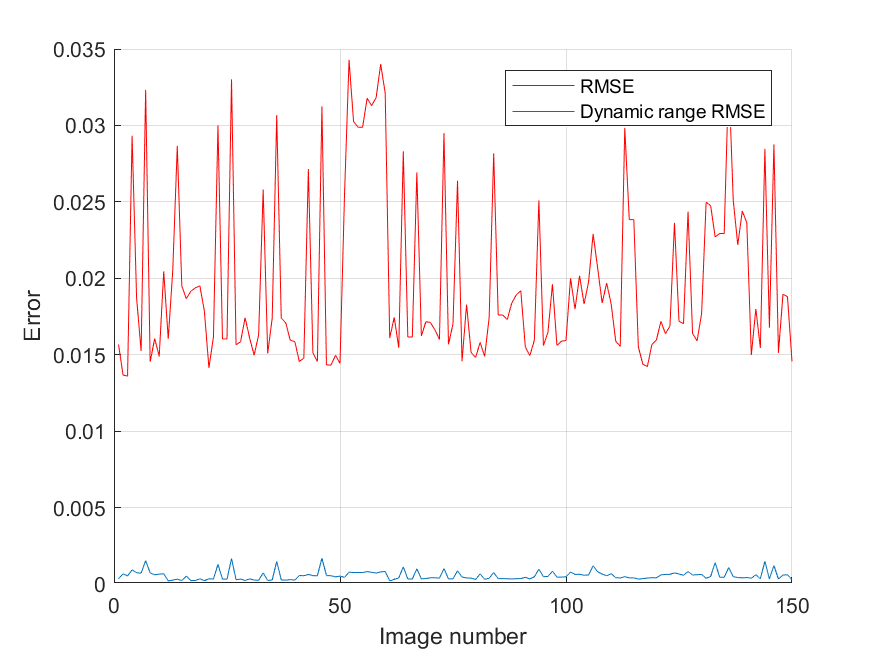
\includegraphics[scale=0.9]{imgs2/rmse_train.png}
	\captionof{figure}{Training set reconstruction errors}
	\label{fig_1}
\end{minipage}
\vskip 0.1in
\begin{minipage}{\linewidth}
	\centering
	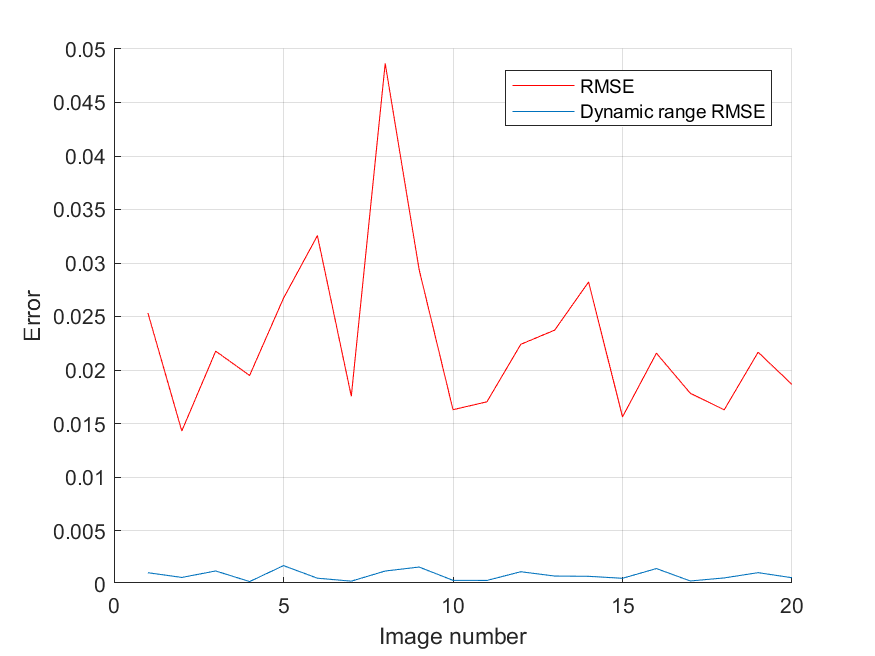
\includegraphics[scale=0.9]{imgs2/rmse_test.png}
	\captionof{figure}{Test set reconstruction errors}
	\label{fig_1}
\end{minipage}
\vskip 0.1in

We can see that the reconstuction errors are larger than the reconstruction from the PCA basis alone from the previous section. We can explain this by the fact the the representation vector from the Section A was of size 25, while in this section we use the representation of size 14.

 \subsection{}
Using the FLD, we achieve a fantastic classification rate of 100\%! This demonstrates that using the Fisher Basis, we achieve better classification of the dataset. The explanation can be found in numerous resources.
\newline
The PCA finds the most accurate representation of the data, in a lower dimensional space. It finds the directions of maximum variances, but those may be not so good for classification, since they may be similar for different classes. What Fisher Linear Discriminator does is finds a projection of the representation of the data, where the classes are separated in an optimal way - where the separation is good. This is done my maximizing the between-classes scatter matrix, and minimizing the within-classes scatter matrix.  Good separation means good classification - there is less overlapping of the classes representations on the projection subspace.


\end{document}




















